% Filename: relatorio.tex
%
% This code is part of 'MT404 2012s2 - Proj04'
% 
% Description: Relatorio do Projeto No.3 de MT404 2012s2.
% 
% Created: 22.08.12 07:25:12 AM
% Last Change: 22.08.12 07:25:12 AM
% 
% Author:
% - Raniere Silva, <r.gaia.cs@gmail.com>
% 
% Copyright (c) 2012, Raniere Silva. All rights reserved.
% 
% Except otherwise noted, this work is licensed under the Creative
% Commons Attribution-ShareAlike 3.0 Unported License. To view a copy of
% this license, visit http://creativecommons.org/licenses/by-sa/3.0/ or
% send a letter to Creative Commons, 444 Castro Street, Suite 900,
% Mountain View, California, 94041, USA.
%
% This work is distributed in the hope that it will be useful, but
% WITHOUT ANY WARRANTY; without even the implied warranty of
% MERCHANTABILITY or FITNESS FOR A PARTICULAR PURPOSE.
%
\documentclass[12pt,a4paper]{article}
% Filename: packages.tex
% 
% This code is part of 'MT404 2012s2'
% 
% Description: This file corresponds to the packages used.
% 
% Created: 22.08.12 07:25:12 AM
% Last Change: 22.08.12 08:23:08 PM
% 
% Authors:
% - Raniere Silva (2012): initial version
% 
% Copyright (c) 2012 Raniere Silva <r.gaia.cs@gmail.com>
% 
% This work is licensed under the Creative Commons Attribution-ShareAlike 3.0 Unported License. To view a copy of this license, visit http://creativecommons.org/licenses/by-sa/3.0/ or send a letter to Creative Commons, 444 Castro Street, Suite 900, Mountain View, California, 94041, USA.
%
% This work is distributed in the hope that it will be useful, but WITHOUT ANY WARRANTY; without even the implied warranty of MERCHANTABILITY or FITNESS FOR A PARTICULAR PURPOSE.
%
\usepackage[utf8]{inputenc}
\usepackage[T1]{fontenc}

% Configura\c{c}\~{o}es regionais
\usepackage[top=3cm,left=2cm,right=2cm,bottom=3cm]{geometry}
\usepackage[brazil]{babel}
\usepackage{indentfirst}

% Pacotes matem\'{a}ticos
\usepackage{amsmath}
\usepackage{amsthm}
\usepackage{amsfonts}
\usepackage{amssymb}
% Customiza\c{c}\~{a}o do pacote amsmath
\newtheorem{defi}{Definição}
\newtheorem{prop}{Proposição}
\newtheorem{teo}{Teorema}
\allowdisplaybreaks[4]

% Pacotes gr\'{a}ficos
\usepackage{graphicx}
\usepackage{tikz}

% Links
\usepackage{url}
\usepackage{hyperref}

% Algoritmos
\usepackage{algorithmic} % Pacote para algoritmos
\usepackage{algorithm} % Pacote para algoritmos
% Customiza\c{c}\~{a}o do pacote algorithm
\floatname{algorithm}{Algoritmo}
\algsetup{linenosize=\small}
\renewcommand{\algorithmicrequire}{\textbf{Entrada:}}
\renewcommand{\algorithmicensure}{\textbf{Saída:}}
\renewcommand{\algorithmicend}{\textbf{fim}}
\renewcommand{\algorithmicif}{\textbf{se}}
\renewcommand{\algorithmicthen}{\textbf{ent\~{a}o}}
\renewcommand{\algorithmicelse}{\textbf{caso contr\'{a}rio}}
\renewcommand{\algorithmicendif}{\algorithmicend}
\renewcommand{\algorithmicfor}{\textbf{para}}
\renewcommand{\algorithmicforall}{\textbf{para todo}}
\renewcommand{\algorithmicdo}{\textbf{fa\c{c}a}}
\renewcommand{\algorithmicendfor}{\algorithmicend}
\renewcommand{\algorithmicwhile}{\textbf{enquanto}}
\renewcommand{\algorithmicendwhile}{\algorithmicend}
\renewcommand{\algorithmicrepeat}{\textbf{repita}}
\renewcommand{\algorithmicuntil}{\textbf{at\'{e}}}
\renewcommand{\algorithmicreturn}{\textbf{retorne}}
\renewcommand{\algorithmiccomment}[1]{\hspace{2em}/* #1 */}

% C\'{o}digos
\usepackage{listings} % Pacote para c\'{o}digos
\usepackage{textcomp} % Para aspas simples
\renewcommand{\lstlistingname}{C\'{o}digo}
\lstdefinestyle{codes}{ %
language=Octave,                % the language of the code
frame=single,                   % frame around the code
basicstyle=\ttfamily\small,     % the size of the fonts that are used for the code
columns=flexible,               % Correct unexpected spaces in strings when copy-and-past
numbers=left,                   % where to put the line-numbers
numberstyle=\footnotesize,      % the size of the fonts that are used for the line-numbers
stepnumber=5,                   % the step between two line-numbers.
numbersep=5pt,                  % how far the line-numbers are from the code
% backgroundcolor=\color{white},  % choose the background color. You must add \usepackage{color}
showspaces=false,               % show spaces adding particular underscores
showstringspaces=false,         % underline spaces within strings
% showtabs=false,                 % show tabs within strings adding particular underscores
% frame=single,                   % adds a frame around the code
tabsize=4,                      % sets default tabsize to 2 spaces
captionpos=t,                   % sets the caption-position to bottom
breaklines=true,                % sets automatic line breaking
breakatwhitespace=false,        % sets if automatic breaks should only happen at whitespace
% caption={\texttt{\lstname}},    % show the filename of files included with \lstinputlisting;
% escapeinside={\%*}{*)},         % if you want to add a comment within your code
% morekeywords={#},               % if you want to add more keywords to the set
upquote=true,                   % Correct single quote
}
\lstdefinestyle{outputs}{ %
language=Octave,                % the language of the code
% frame=single,                   % frame around the code
basicstyle=\ttfamily\small,     % the size of the fonts that are used for the code
columns=flexible,               % Correct unexpected spaces in strings when copy-and-past
% numbers=left,                   % where to put the line-numbers
% numberstyle=\footnotesize,      % the size of the fonts that are used for the line-numbers
% stepnumber=5,                   % the step between two line-numbers.
% numbersep=5pt,                  % how far the line-numbers are from the code
% backgroundcolor=\color{white},  % choose the background color. You must add \usepackage{color}
showspaces=false,               % show spaces adding particular underscores
showstringspaces=false,         % underline spaces within strings
% showtabs=false,                 % show tabs within strings adding particular underscores
% frame=single,                   % adds a frame around the code
tabsize=4,                      % sets default tabsize to 2 spaces
% captionpos=t,                   % sets the caption-position to bottom
breaklines=true,                % sets automatic line breaking
breakatwhitespace=false,        % sets if automatic breaks should only happen at whitespace
% caption={\texttt{\lstname}},    % show the filename of files included with \lstinputlisting;
% escapeinside={\%*}{*)},         % if you want to add a comment within your code
% morekeywords={#}                % if you want to add more keywords to the set
upquote=true,                   % Correct single quote
}

% Novos comandos

\begin{document}
\title{Projeto No.4 de MT404}
\author{Raniere Silva \\ ra092767}
\maketitle
\begin{abstract}
    Este \'{e} o projeto no.4 da disciplina MT404 - M\'{e}todos Computacionais
    de \'{A}lgebra Linear. Neste projeto utilizamos a função interna do GNU
    Octave para calcular a fatoração LU de uma matriz para investigar a perda de
    esparsidade no fatores $L$ e $U$ e a possibilidade de minimizar essa perda.

    Verificou-se, computacionalmente, que realmente é possível preservar parte
    da esparsidade de uma matriz ao calcular a fatoração LU mas existe um limite
    para essa possibilidade. Também verificou-se que a tentativa de preservar a
    esparcidade não produz alteração significativa no erro e nem no tempo de
    execução para a solução de um sistema linear.
\end{abstract}
\tableofcontents
\lstlistoflistings
\section*{Licen\c{c}a}
Salvo disposi\c{c}\~{a}o em contr\'{a}rio, este trabalho foi licenciado com uma
Licen\c{c}a Creative Commons Atribui\c{c}\~{a}o - CompartilhaIgual 3.0 N\~{a}o
Adaptada. Para ver uma c\'{o}pia desta licen\c{c}a, visite
http://creativecommons.org/licenses/by-sa/3.0/.
\begin{center}
    
\includegraphics{../figuras/cc-by-sa.png}
\end{center}
\newpage
\section{Fatora\c{c}\~{a}o LU}
A maneira mais elementar de resolver um sistema de equa\c{c}\~{o}es \'{e} \'{e}
utilizando a elimina\c{c}\~{a}o de Gauss, i.e., em triangularizar o
sistema, e posteriormente utilizar substitui\c{c}\~{a}o para obter a
solu\c{c}\~{a}o do sistema.

A Fatora\c{c}\~{a}o LU \'{e} uma vers\~{a}o mais elaborada da elimina\c{c}\~{a}o
de Gauss e dado o sistema $A x = b$ encontrar matrizes $L$ e $U$, onde $L$ \'{e}
tringular inferior com diagonal unit\'{a}ria e $U$ triangular superior, tal que
$A = L U$. A solu\c{c}\~{a}o do sistema linear \'{e} obtida resolvendo dois
sistemas:
\begin{align*}
    L y &= b, \\
    U x &= y.
\end{align*}

\'{E} poss\'{i}vel provar que $A \in \mathbb{R}^{n \times n}$ possue
fatora\c{c}\~{a}o LU se os menores principais de $A$, de ordem $1, 2, \ldots, n
- 1$, s\~{a}o n\~{a}o nulos. Al\'{e}m disso, se a fatora\c{c}\~{a}o existir e
$A$ for n\~{a}o singular, ent\~{a}o a fatora\c{c}\~{a}o LU \'{e} \'{u}nica.

Sabe-se que para algumas matrizes n\~{a}o \'{e} poss\'{i}vel obter a
fatora\c{c}\~{a}o LU, e.g.,
\begin{align*}
    A = \begin{bmatrix}
        0 & 1 \\
        1 & 0
    \end{bmatrix}.
\end{align*}
Para algumas dessas matrizes, existe uma matriz $P$, $P$ \'{e} uma matriz de
permuta\c{c}\~{a}o, tal que existe a fatora\c{c}\~{a}o LU de $P A$.

A matriz $P$ pode ser calculada durante a tentativa de calcular a fatoração LU
de $A$ uma vez que precisa-se permutar duas linhas de $A$ apenas quando
encontra-se um pivô igual zero. O uso de uma matriz $P$ também pode tornar a
fatoração LU mais estável. Por esses motivos, todas as implementações da
fatoração LU utilizam permutações (parcial e/ou total).

No caso de matrizes esparsas, a fatora\c{c}\~{a}o LU pode causar o preenchimento
da matrizes $L$ e $U$, para evitar isso pode-se relaxar a permuta\c{c}\~{a}o
$P$.

\section{Experimentos Computacionais}
O GNU Octave possue implementado, no arquivo lu.oct, uma fun\c{c}\~{a}o para o c\'{a}lculo da
fatora\c{c}\~{a}o LU de uma matriz. Essa fun\c{c}\~{a}o recebe como
par\^{a}metro a matriz $A$ que deseja-se calcular os fatores $L$ e $U$ e,
opcionalmente, um escalar $\mathrm{THRESH}$, $0 < \mathrm{THRESH} \leq 1$, que
define uma toler\^{a}ncia na escolha do piv\^{o} a ser utilizado na tentativa de
minimizar o preenchimento nas matrizes $L$ e $U$.

Intuitivamente, propomos as seguintes hipóteses ao manter a dimensão da matriz
constante:
\begin{enumerate}
    \item ao diminuir o valor de $\mathrm{THRESH}$ a esparcidade de $L$ e $U$
        aumenta (devido a toler\^{a}ncia na escolha do piv\^{o});
        \label{hip:esp}
    \item o tempo para calcular a fatora\c{c}\~{a}o LU com $\mathrm{THRESH} = 1$
        seja inferior as demais (devido a realizar apenas uma conparação);
        \label{hip:thres1}
    \item ao diminuir o valor de $\mathrm{THRESH}$ o tempo tamb\'{e}m diminua
        (pela redu\c{c}\~{a}o no n\'{u}mero de opera\c{c}\~{o}es);
        \label{hip:tempo}
    \item a precis\~{a}o da solu\c{c}\~{a}o seja superior quanto mais alto for o
        valor de $\mathrm{THRESH}$ (por questão de estabilidade na escolha do
        pivô). \label{hip:est}
\end{enumerate}

Para testar as hipóteses acima, implementou-se as funções definidas no
Código~\ref{code:mt404_p04} e o script do Código~\ref{code:call_mt404_p04}.

O Código~\ref{code:call_mt404_p04} produz algumas figuras, dentre elas as
Figuras~\ref{fig:dim100}~\ref{fig:dim200}~e~\ref{fig:dim400} que ilustram o
prenchimento dos fatores $L$ e $U$ de uma matriz $A$ em função da densidade da
matriz $A$ e do valor do parâmetro $\mathrm{THRESH}$. Nessas três figuras, a
matriz $A$ é representada pelos pontos mais claros e as matrizes $L$ e $U$ pelos
pontos mais escuros\footnote{A representação da matriz $A$ foi sobreposta à
representação das matrizes $L$ e $U$ de modo que perdeu-se um pouco de
informação. Entretanto é válido supor que os elementos não nulos em $A$ não
foram zerados.}. Ainda nessas três figuras, a densidade da matriz $A$ diminui de
cima para baixo e o valor de $\mathrm{THRESH}$ diminui da esquerda para a
direita.
\begin{figure}[!htb]
    \begin{center}
        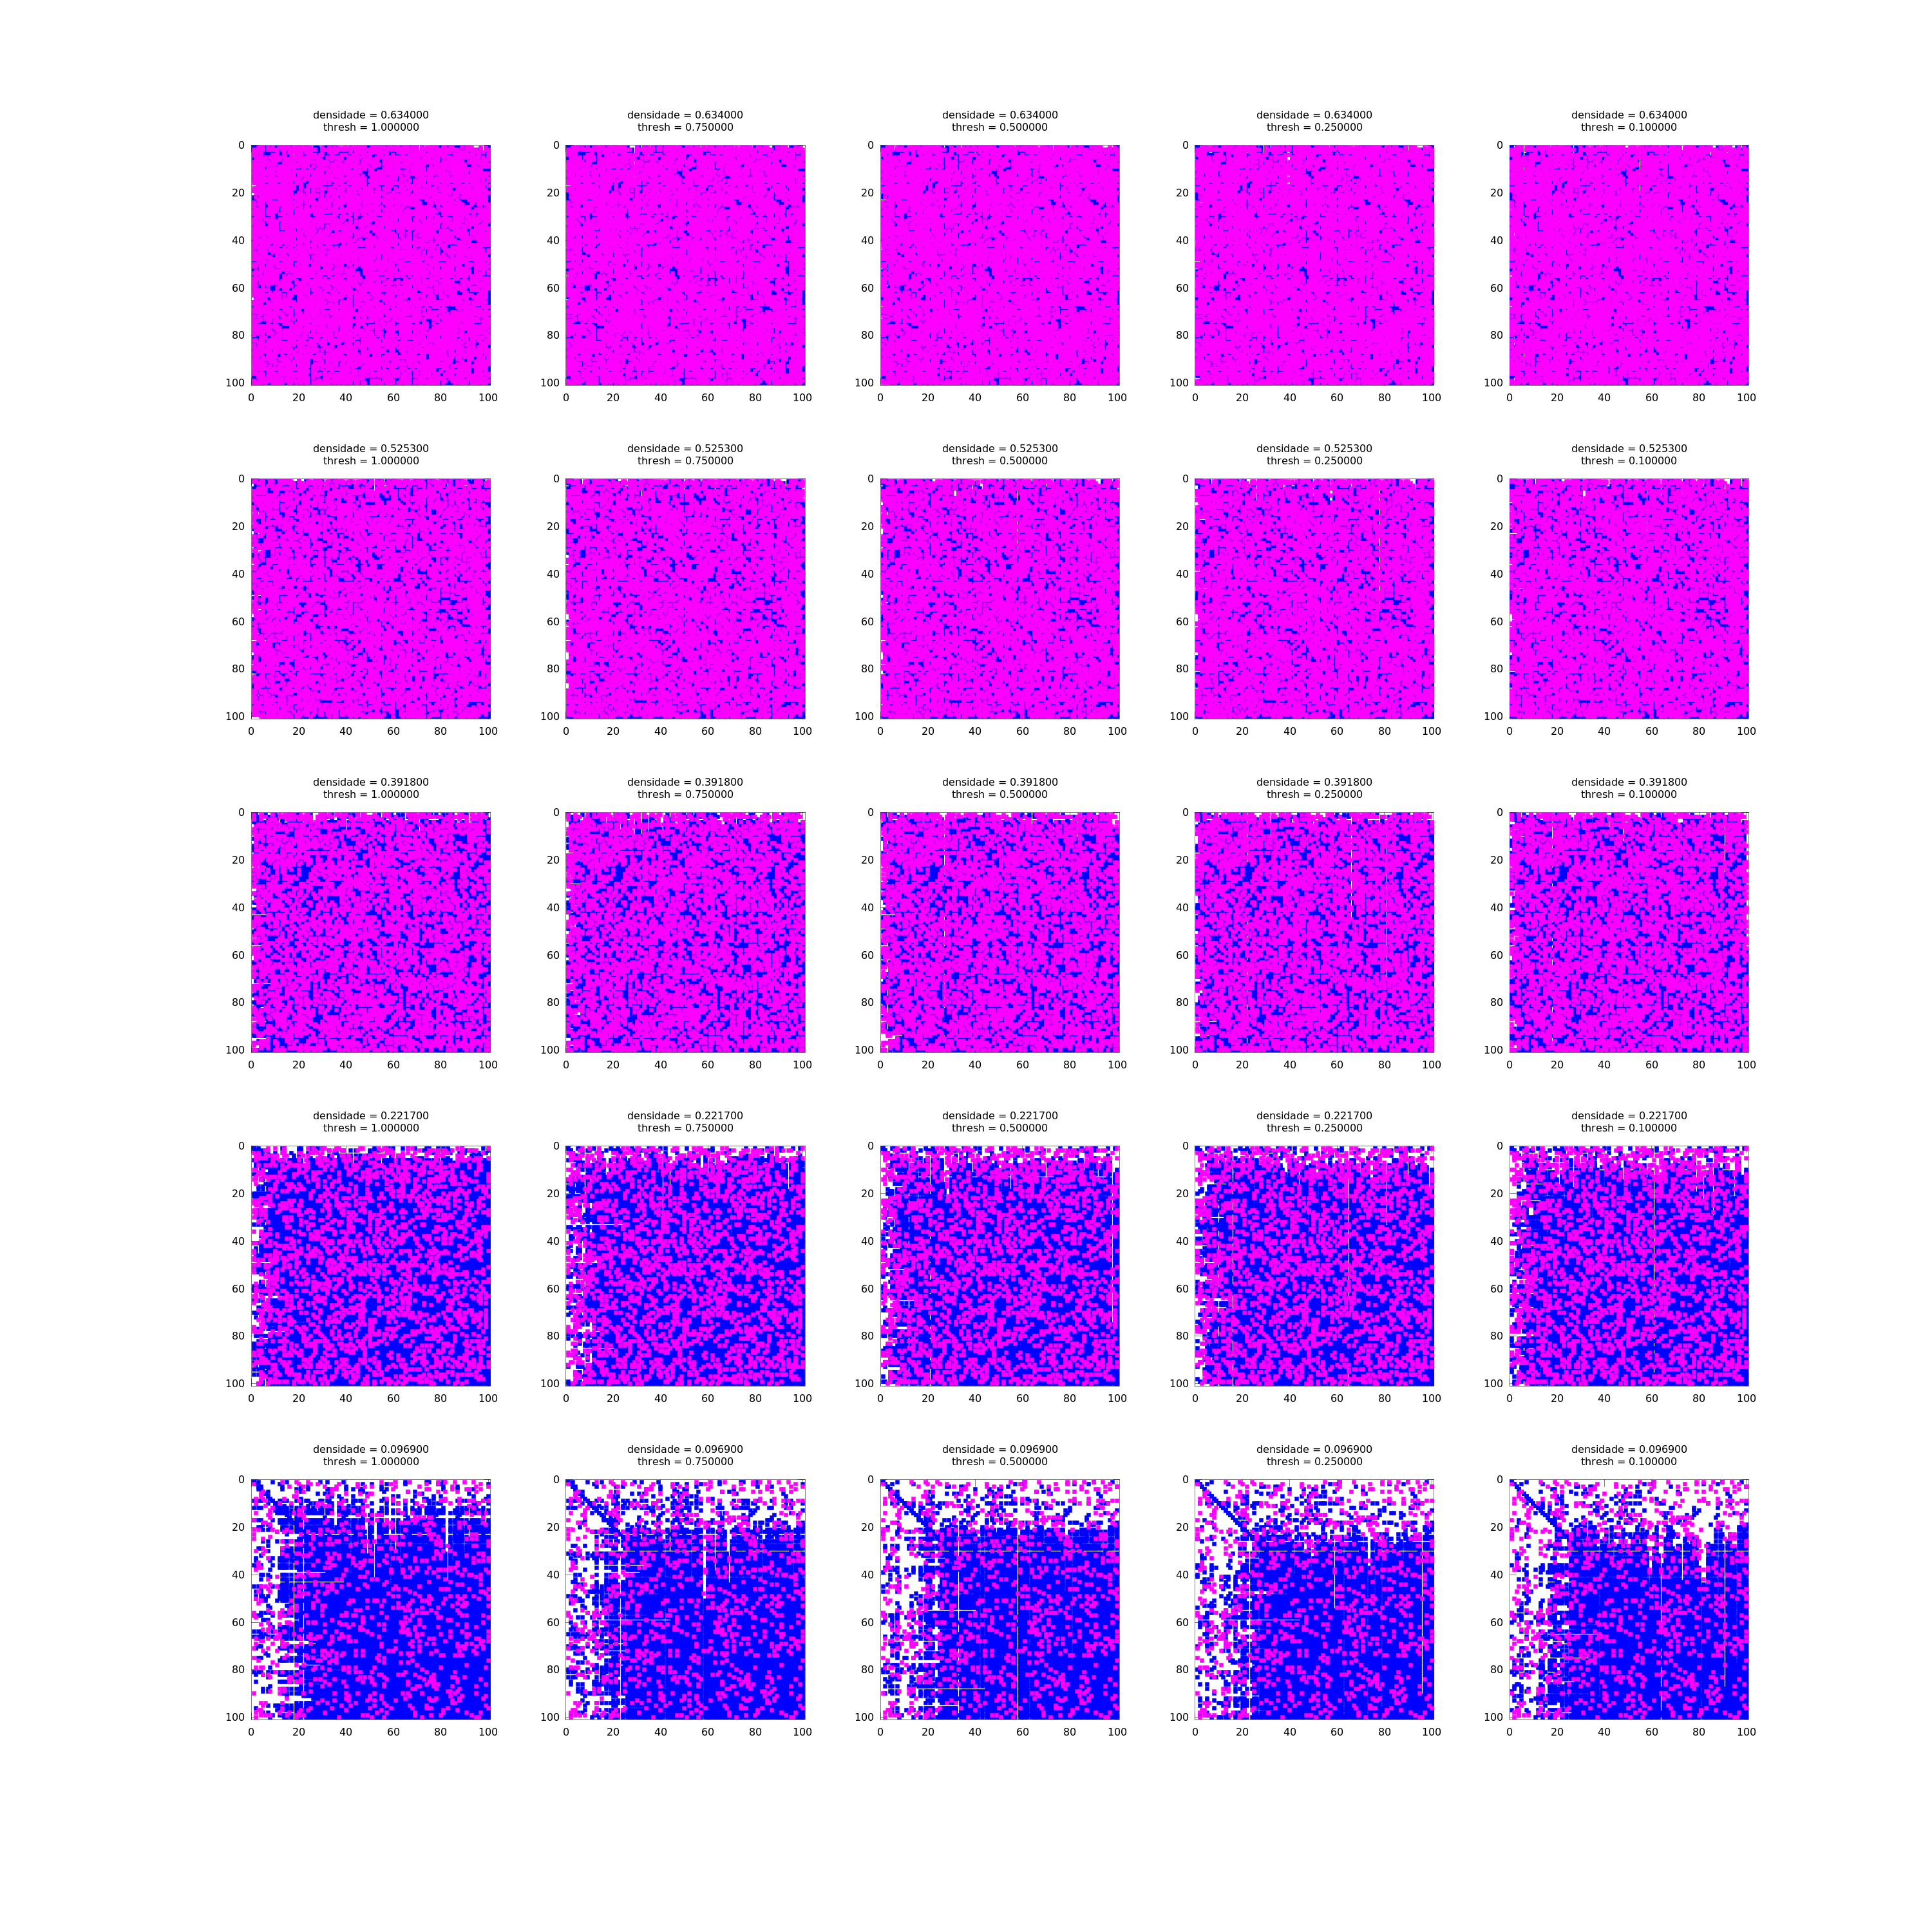
\includegraphics[width=\textwidth, trim=300 300 250 100, clip]{src/dim100.png}
    \end{center}
    \caption{Ilustração comparativa da esparcidade dos fatores $L$ e $U$ de uma
    matriz $A$.}
    \label{fig:dim100}
\end{figure}
\begin{figure}[!htb]
    \begin{center}
        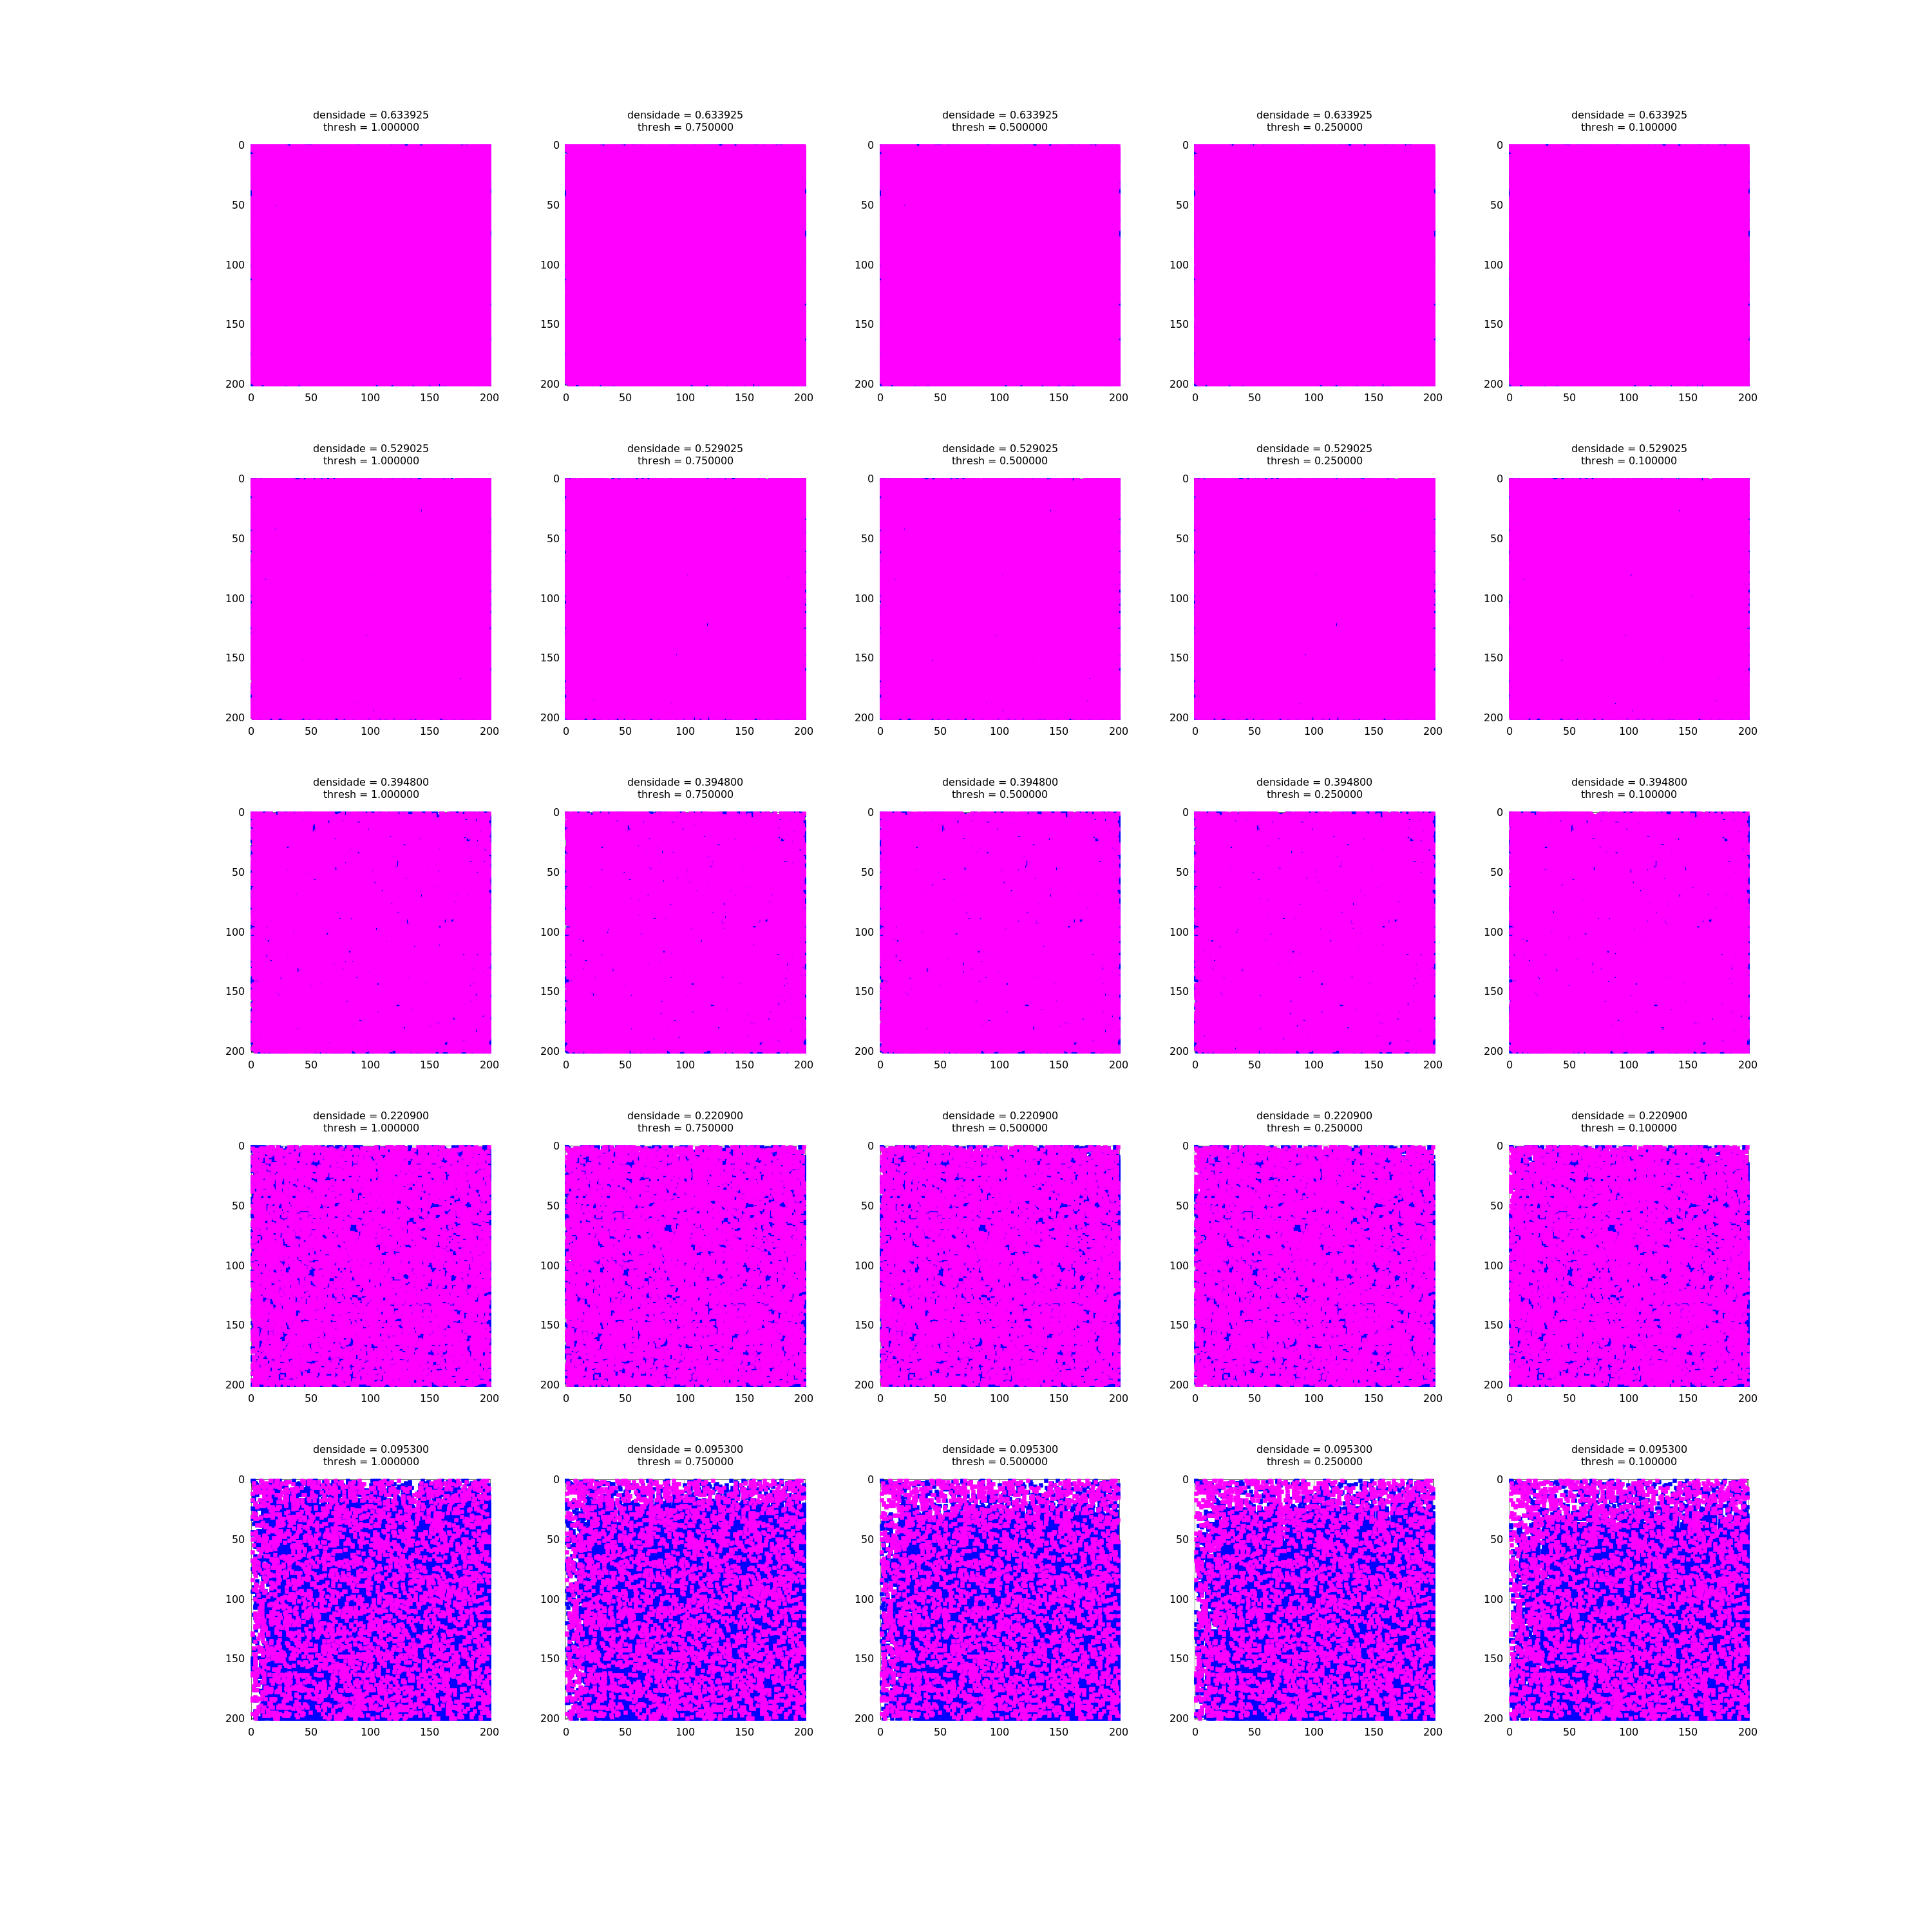
\includegraphics[width=\textwidth, trim=300 300 250 100, clip]{src/dim200.png}
    \end{center}
    \caption{Ilustração comparativa da esparcidade dos fatores $L$ e $U$ de uma
    matriz $A$.}
    \label{fig:dim200}
\end{figure}
\begin{figure}[!htb]
    \begin{center}
        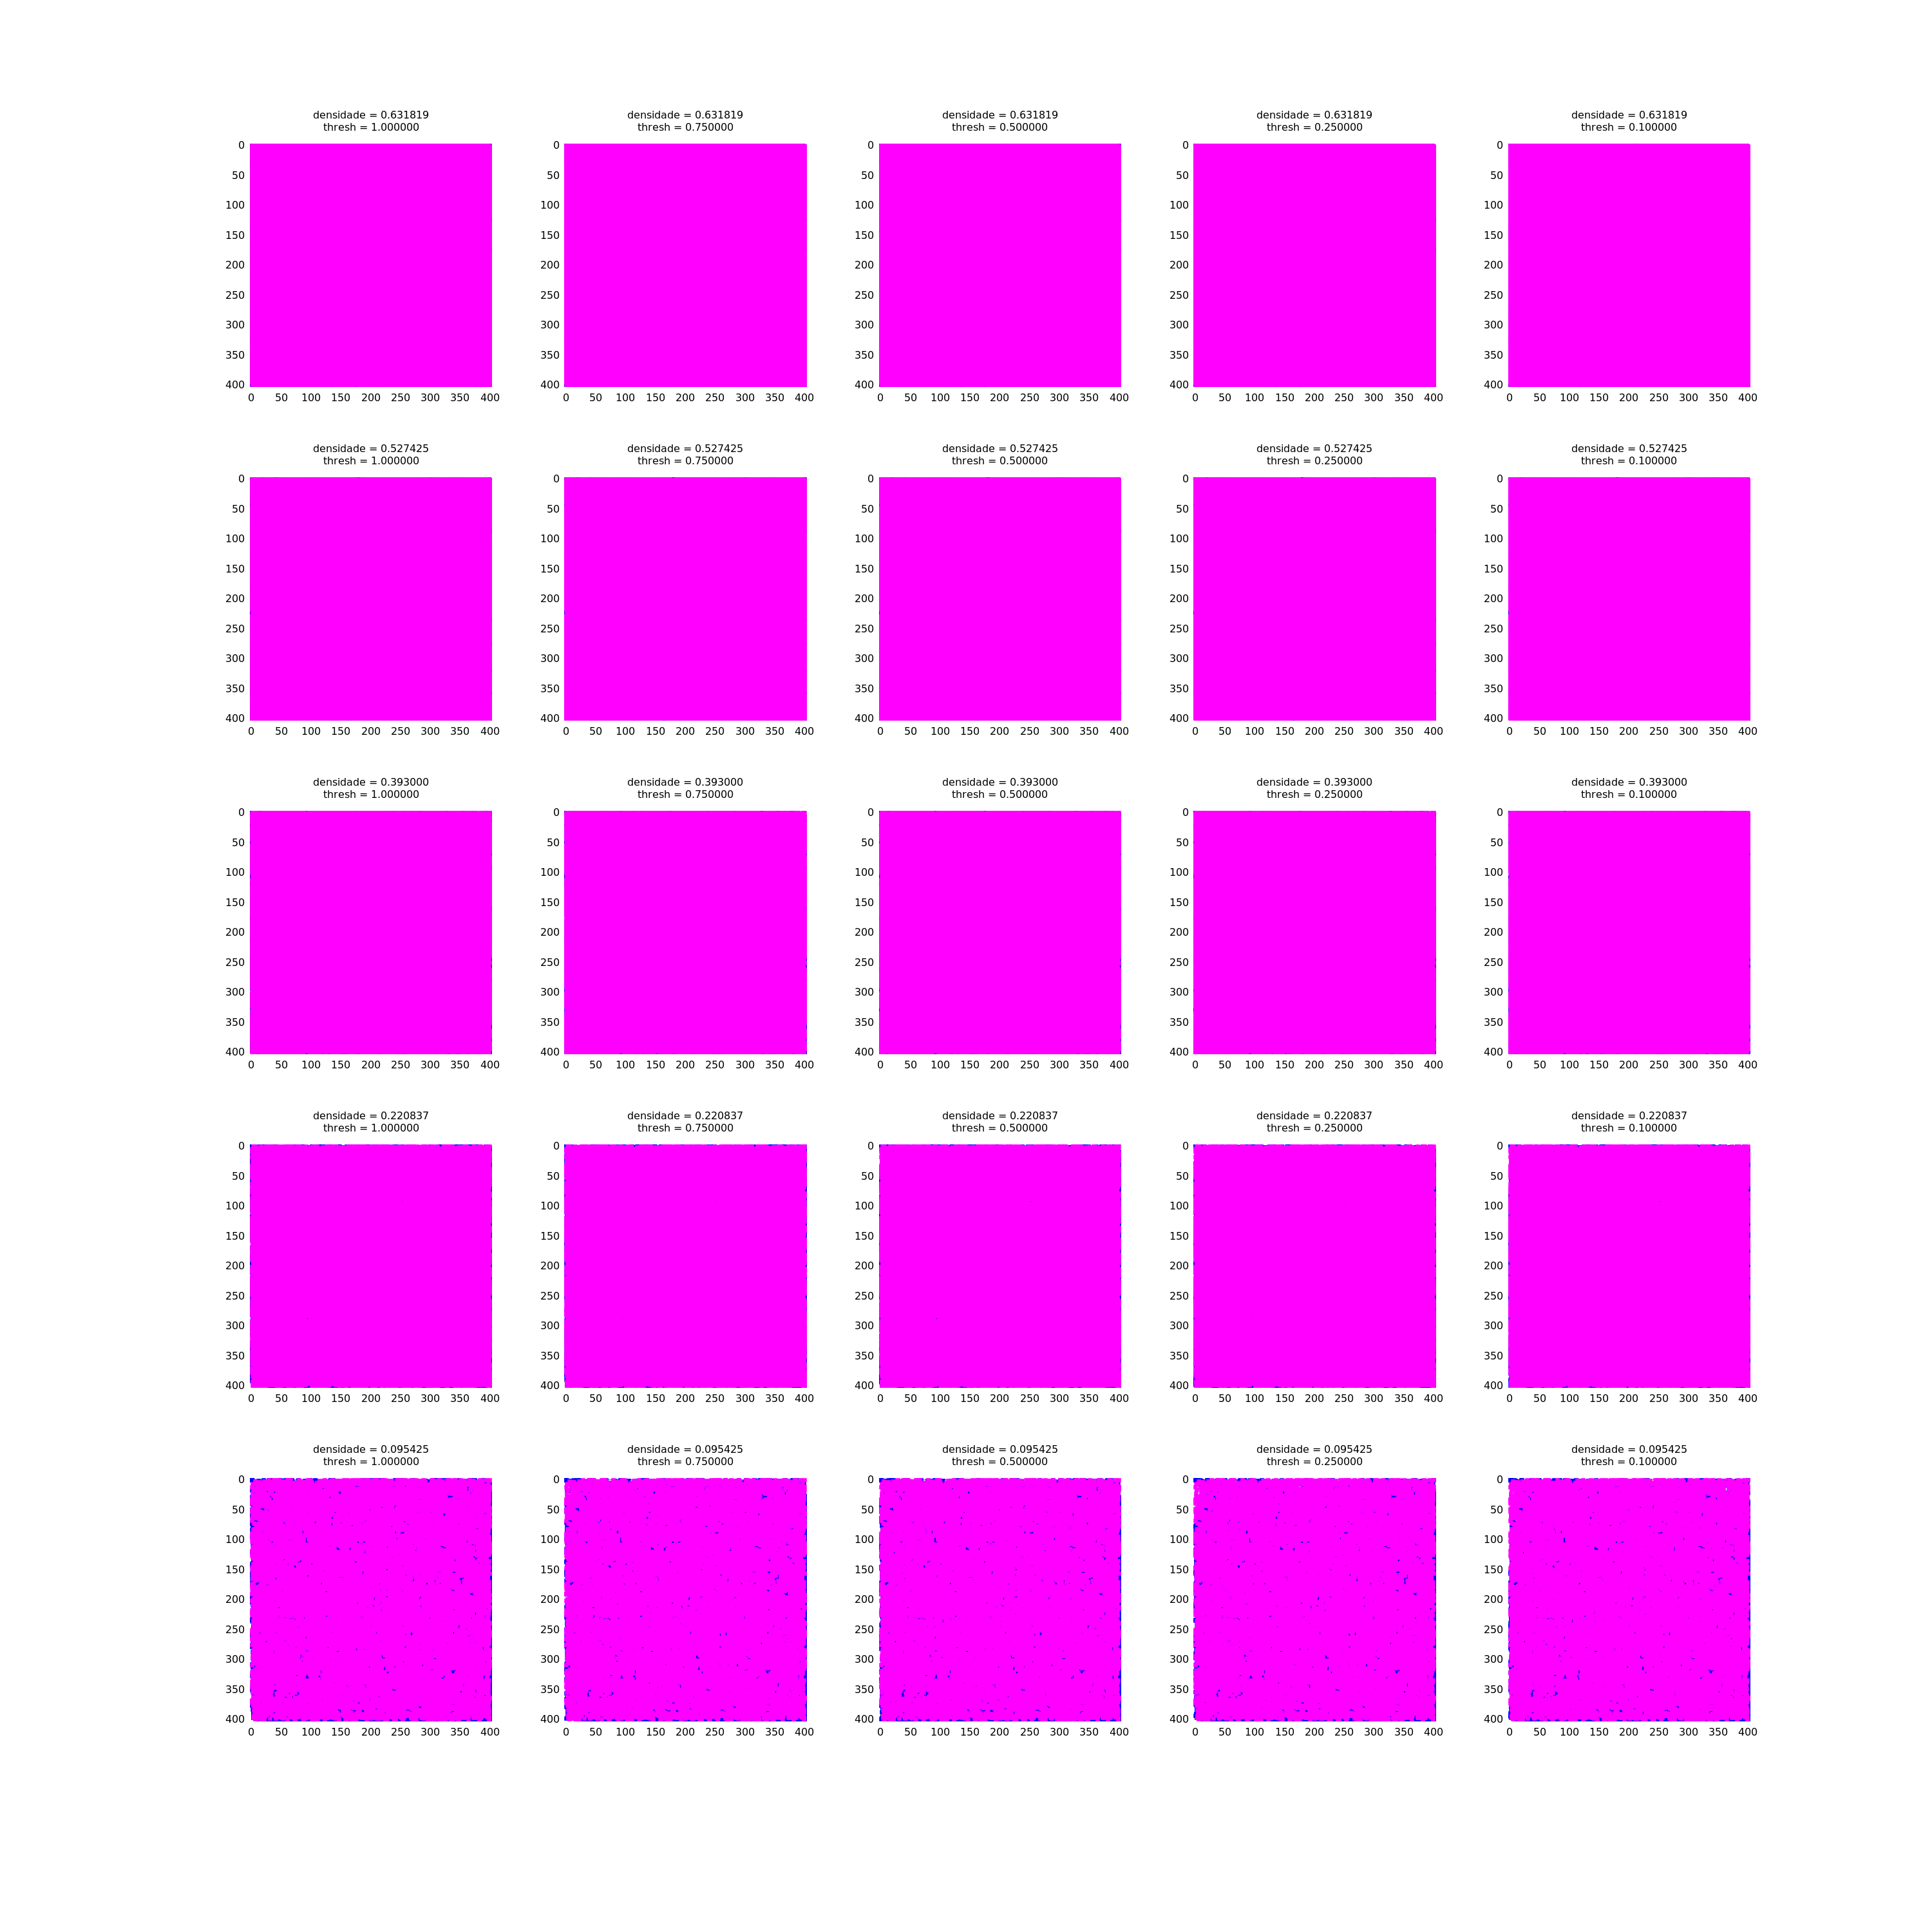
\includegraphics[width=\textwidth, trim=300 300 250 100, clip]{src/dim400.png}
    \end{center}
    \caption{Ilustração comparativa da esparcidade dos fatores $L$ e $U$ de uma
    matriz $A$.}
    \label{fig:dim400}
\end{figure}

Observando a Figura~\ref{fig:dim100}, verificamos o preenchimento nos fatores
$L$ e $U$. Embora esse fenômeno esteja presente independentente da densidade da
matriz $A$ e do valor de $\mathrm{THRESH}$ ele é mais visível quando a densidade
da matriz $A$ é pequena, caso da última linha. Na última linha, observamos que
ao diminuir o valor de $\mathrm{THRESH}$ a esparcidade dos fatores $L$ e $U$
aumenta (isso indica que nossa hipótese~\ref{hip:esp} pode estar correta).

Esperava-se que as Figuras~\ref{fig:dim200}~e~\ref{fig:dim400} apresentassem
comportamento semelhante a da Figura~\ref{fig:dim100} o que, visualmente, não
ocorre. Para testar se o tamanho das Figuras~\ref{fig:dim200}~e~\ref{fig:dim400}
está comprometendo a análise do experimento, modificamos o tamanho da figura,
ver Figura~\ref{fig:zoom}, e verificamos que era o tamanho da imagem que
impossibilitava de visualizar a perda da esparsidade. 
\begin{figure}[!htb]
    \begin{center}
        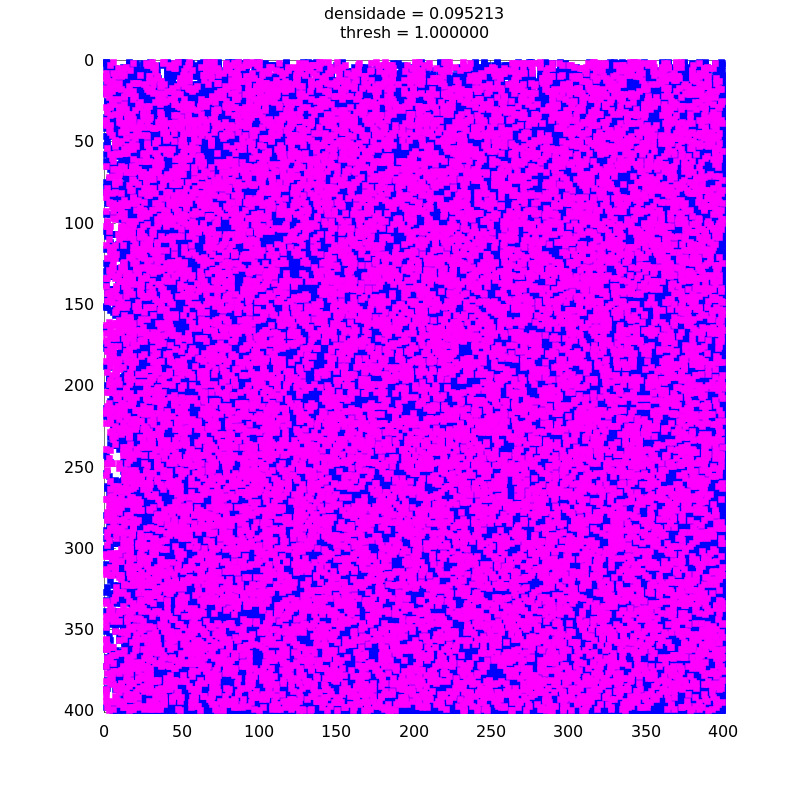
\includegraphics[width=.4\textwidth, trim=300 300 250 100,
        clip]{src/zoom400-3-1.png}
        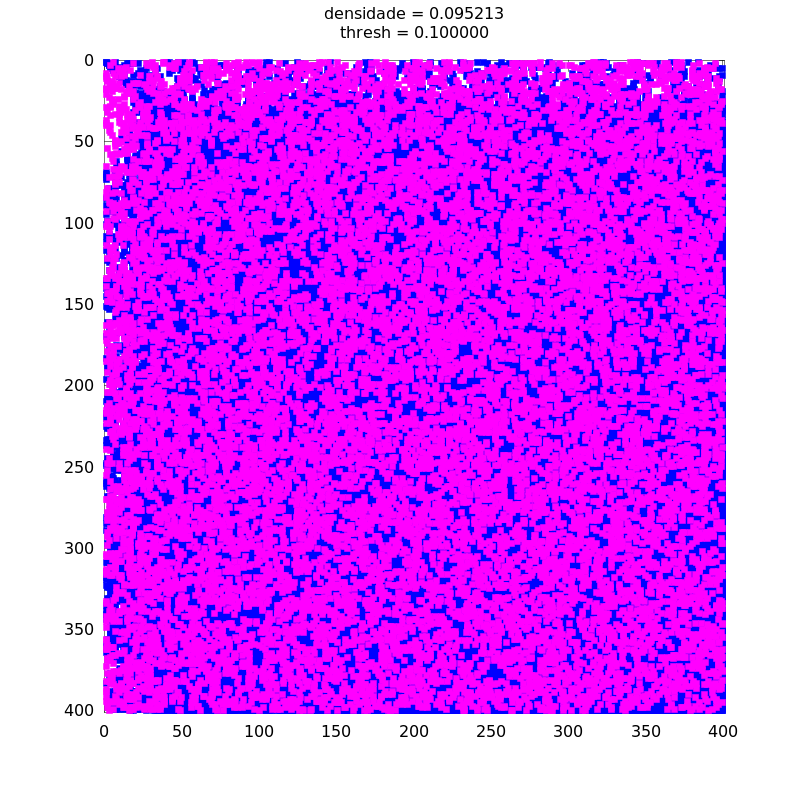
\includegraphics[width=.4\textwidth, trim=300 300 250 100,
        clip]{src/zoom400-3-5.png}
    \end{center}
    \caption{Ilustração comparativa da esparcidade dos fatores $L$ e $U$ de uma
    matriz $A$ de dimensão $400$, densidade próxima de $10\%$ e valor de
    $\mathrm{THRESH}$ igual a $1$ (esquerda) e de $0,1$ (direita).}
    \label{fig:zoom}
\end{figure}

Ao testar vários valores para $\mathrm{THRESH}$, observou-se que ao diminuir o
valor de $\mathrm{THRESH}$ para menos que $0.1$ a esparsidade dos fatores $L$ e
$U$ não diminui mui mais que a esparcidade obtida ao utilizar $\mathrm{THRESH} =
0.1$. Na Figura~\ref{fig:sparse} ilustramos essa observação.
\begin{figure}[!htb]
    \begin{center}
        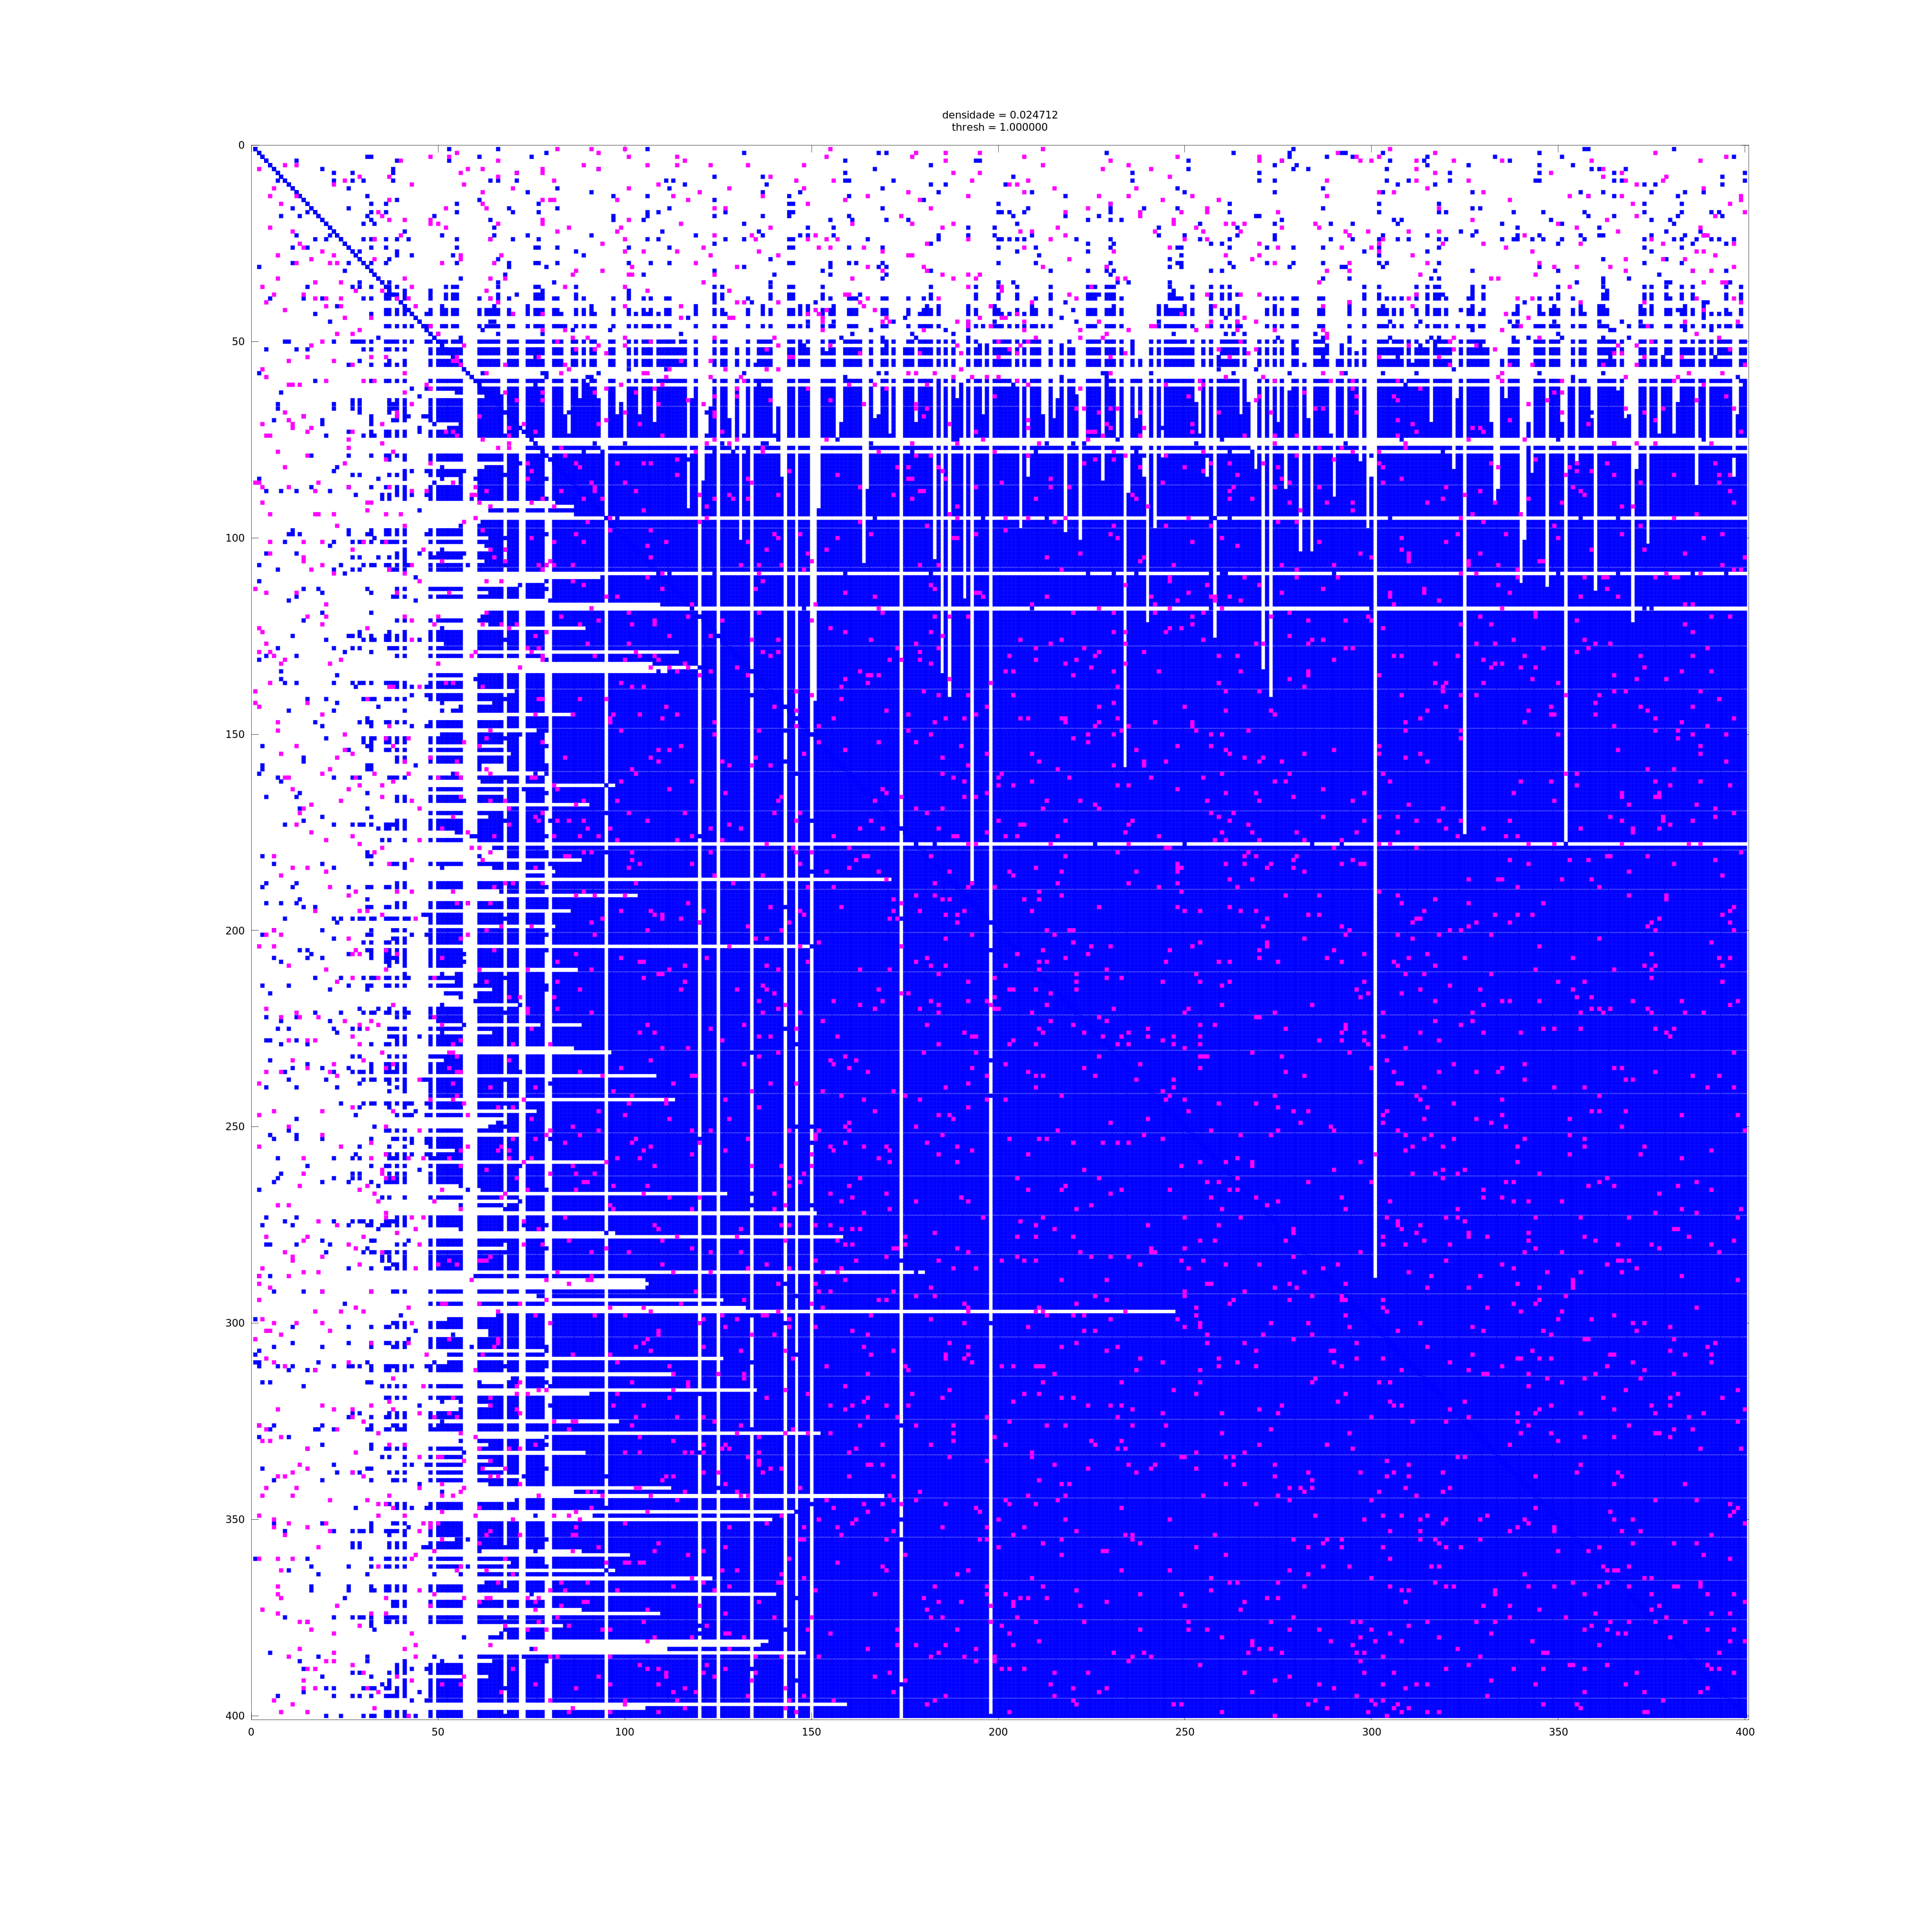
\includegraphics[width=.3\textwidth, trim=300 300 250 100,
        clip]{src/sparse400-2-1.png}
        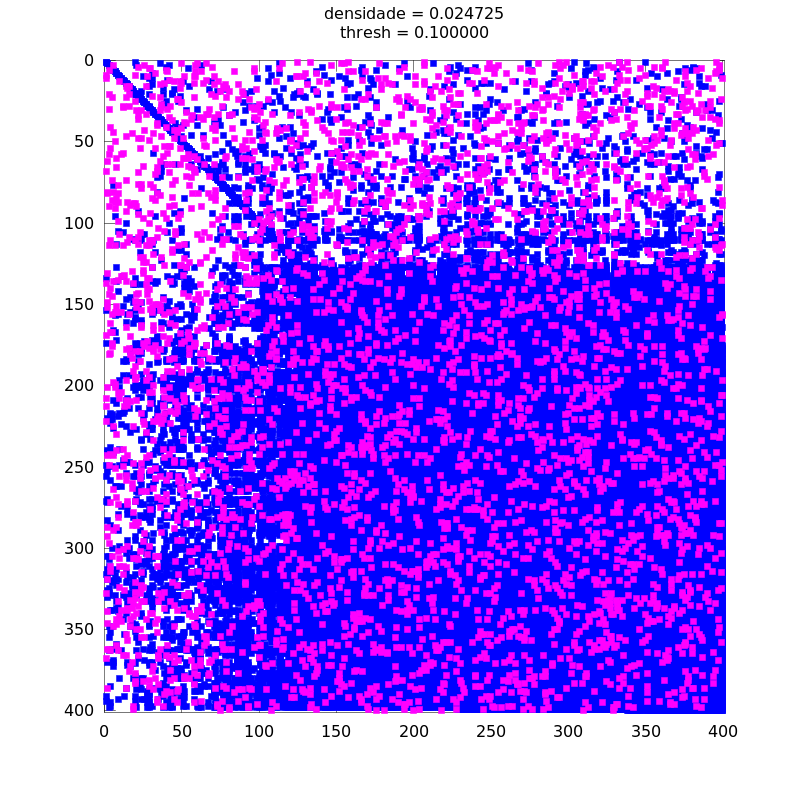
\includegraphics[width=.3\textwidth, trim=300 300 250 100,
        clip]{src/sparse400-2-5.png}
        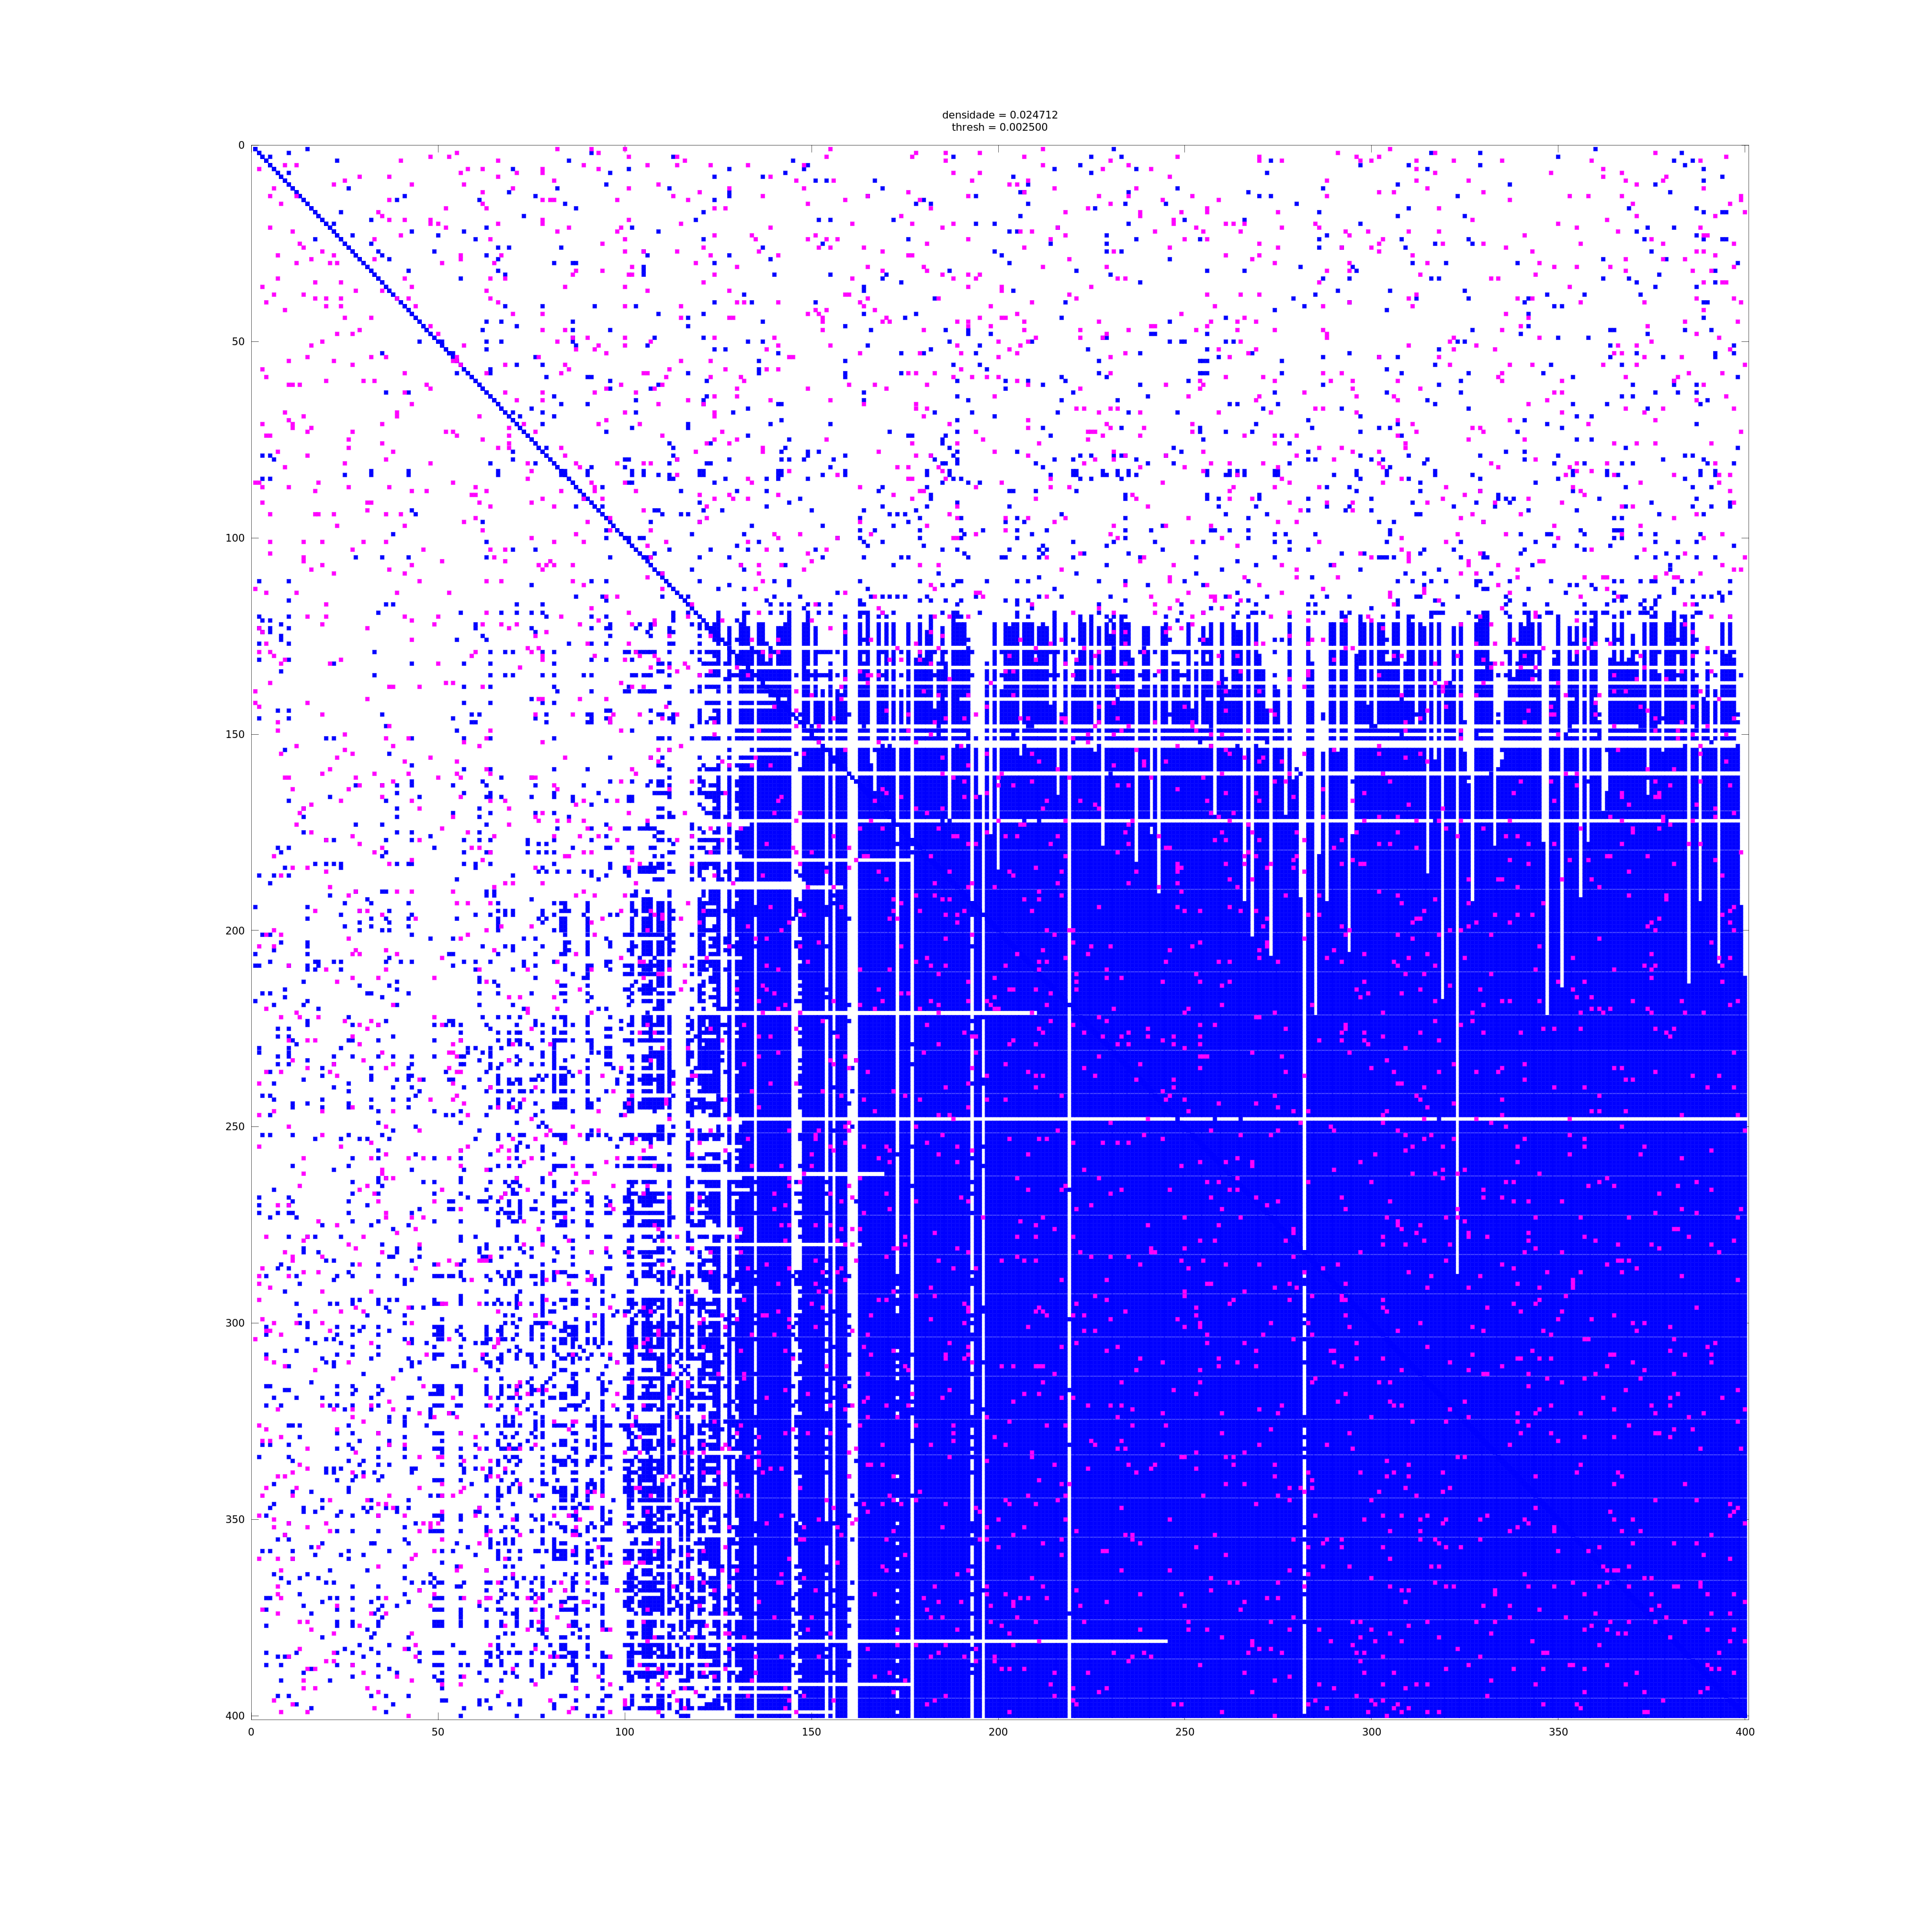
\includegraphics[width=.3\textwidth, trim=300 300 250 100,
        clip]{src/sparse400-2-10.png}
    \end{center}
    \caption{Ilustração comparativa da esparcidade dos fatores $L$ e $U$ de uma
    matriz $A$ de dimensão $400$, densidade próxima de $2.5\%$ e valor de
    $\mathrm{THRESH}$ igual a $1$ (esquerda), $0,1$ (centro) e $0.025$ (direita).}
    \label{fig:sparse}
\end{figure}

Em relação ao erro relativo e ao tempo para resolver um sistema linear, estes
não sofreram grande modificação ao modificar o valor do $\mathrm{THRESH}$
(nossas hipóteses~\ref{hip:thres1}~-~\ref{hip:est} mostraram-se falsas). A
Tabela~\ref{tab:info400} representa o comportamento geral do erro e do tempo
para uma dada dimensão ao variar o valor do $\mathrm{THRESH}$.
\input{table.csv}

\clearpage
\section{C\'{o}digos}
A seguir encontra-se os c\'{o}digos desenvolvidos neste projeto. Todos os c'{o}digos
foram testados utilizando o GNU Octave em sua vers\~{a}o
3.2.4\footnote{Acredita-se que os c\'{o}digos sejam compat\'{i}eis com o MATLAB
embora n\~{a}o tenham sido testados nesse ambiente.} e encontram-se
dispon\'{i}veis em \url{https://github.com/r-gaia-cs/mt404-2012s2}.
\lstinputlisting[style=codes, caption={An\'{a}lise de sensibilidade},
label={code:mt404_p04}]{src/mt404_p04.m}
\lstinputlisting[style=codes, caption={Testes executados},
label={code:call_mt404_p04}]{src/call_mt404_p04.m}
\end{document}
